\section{Uppgift 10}\label{uppgift-10}

\subsection{Instruktioner}
\begin{verbatim}
10. Skriv ett program där användaren ska ange ordningsnumret på en månad (1-12).
    Programmet ska sedan skriva ut månadens namn och antal dagar. Om man anger
    felaktigt månadsnummer (mindre än 0 eller större än 12) så ska ett
    felmeddelande skrivas på skärmen, och man ska sedan kunna ange ett nytt
    nummer. Använd switch-sats i din lösning

    Programmet ska fortsätta att fråga efter månadsnummer ända tills man har
    matat in 0 (noll). Då ska programmet avbrytas.
\end{verbatim}


\subsection{Lösning}
\subsubsection{Funktion}
% TODO: Funktion på #10.
\subsubsection{Kommentar}
% TODO: Kommentar på #10.

\subsubsection{Källkod}\label{uppgift-10_src}
%\begin{listing}[H]
    \inputminted[linenos]{java}{src/Lab1Uppg10.java}
    \caption{Lab1Uppg10.java}
    \label{Uppg10src}
%\end{listing}

\subsubsection{Skärmdump}
\begin{figure}[htbp]
    \centering
        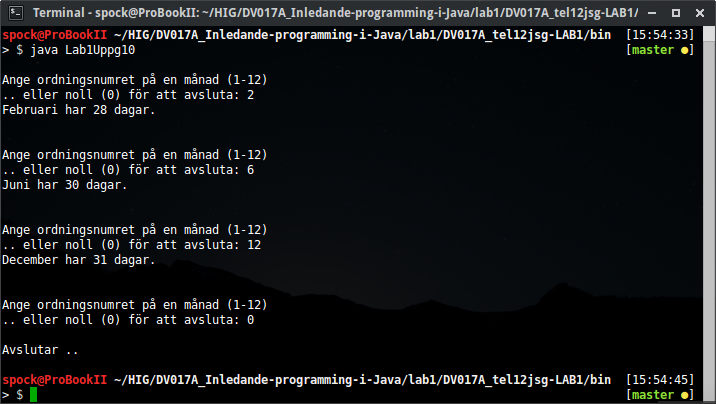
\includegraphics[width=\linewidth]{img/10.png}
    \caption{Körning av koden till Uppgift \ref{uppgift-10}}
    \label{fig:screenshot-10}
\end{figure}
